\documentclass[12pt, a4paper]{article}

\usepackage[utf8]{inputenc}
\usepackage{mathtools}
\usepackage{amssymb}
\usepackage{ntheorem}
\usepackage[framemethod=TikZ]{mdframed}
\usepackage{amsmath}
\usepackage[hidelinks]{hyperref}
\usepackage{cleveref}
\usepackage[most]{tcolorbox}
\usepackage{fancyhdr}
\usepackage{lastpage}
\usepackage{geometry}
\usepackage{graphicx}
\usepackage{float} 
\usepackage{subfigure} 
\usepackage{arydshln}
\usepackage{multicol}
\usepackage{url}
\usepackage{setspace}
\usepackage[T1]{fontenc}
\usepackage{mathptmx}
%\usepackage{draftwatermark}

\geometry{a4paper, left=2cm, right=2cm, bottom=2cm, top=2cm}

\definecolor{blue}{rgb}{0,0.45,1.14}
\definecolor{red}{rgb}{0.77,0.12,0.23}
\definecolor{grey}{rgb}{0.49,0.38,0.29}
\definecolor{green}{rgb}{0,0.42,0.24}
\definecolor{SpringGreen}{rgb}{0.95,0.97,0.95}
\definecolor{OliverGreen}{rgb}{0.09,0.34,0.09}
\definecolor{LeftGreen}{rgb}{0.13,0.54,0.13}
\definecolor{orange}{rgb}{2.07,0.69,0.32}

%\SetWatermarkText{Initial Draft} % the Text
%\SetWatermarkLightness{0.9} % the lightness from 0 to 1, default 0.8
%\SetWatermarkScale{1.0} % the scale, default 1.2

\theorembodyfont{\rmfamily}
\newtheorem{theorem}{Theorem}[subsection]
\newtheorem{definition}{Definition}[subsection]
\newtheorem{example}{Example}[subsection]
\newtheorem{proof}{Proof}[subsection]
\newtheorem{axiom}{Axiom}[subsection]

\rhead{\thepage}
\linespread{1.15}

\title{\textbf{IB Mathematics Analysis and Approaches HL}\\
Topic 4 Probability}
\author{Jiuru Lyu}
\date{\today}

\def\Z{{\mathbb{Z}}}
\def\R{{\mathbb{R}}}
\def\C{{\mathbb{C}}}
\def\Q{{\mathbb{Q}}}
\def\E{{\mathbb{E}}}
\def\d{{\mathrm{d}}}
\def\i{{\mathrm{i}}}
\def\RE{{\mathrm{Re}}}
\def\IM{{\mathrm{Im}}}
\def\Arg{{\mathrm{Arg}}}
\def\cis{\mathrm{cis}}
\def\P{\mathrm{P}}
\def\Var{\mathrm{Var}}
\def\E{\mathrm{E}}

\begin{document}

\maketitle
\tableofcontents

\newpage

\section{Statistics and Probability}
\subsection{An Introduction to Statistics}
\begin{enumerate}
    \item Statistical inferences: when the sample data is well chosen and described, an analysis will allow us to draw conclusions about the population based on this sample. 
    \begin{itemize}
        \item \textbf{\color{red}{Discrete data}} is data that can be counted; it gives the number of times something occurs or the number of items that exists.
        \item \textbf{\color{red}{Continuous data}} is data that is measured; however, the values of the actual data cannot be determined exactly, and the data may be limited to a range.
    \end{itemize}
    \item Reliability and Bias. 
    \item Data Sampling (Sampling Methods): 
    \begin{itemize}
        \item \textbf{Simple}: Achieving randomness by a simple, completely random process.
        \item \textbf{Convenience}: Choosing a sample based on how easy it is to find the data. 
        \item \textbf{Systematic}: If data is listed, selecting a random starting point and then choosing the rest of the sample at a consistent interval in the list. 
        \item \textbf{Quota}: Choosing a sample that is only comprised of members of the population that fit certain characteristics. 
        \item \textbf{Satisfied}: Choosing a random sample in a way that the population of certain characteristics matches the proportion of those characteristics in the population. 
    \end{itemize}
    \item Grouped Data: 
    \begin{itemize}
        \item Key terms: intervals/classes, frequency distribution table, frequency diagram. 
        \item Frequency diagram of discrete data: 
        \begin{figure}[H]
            \center
            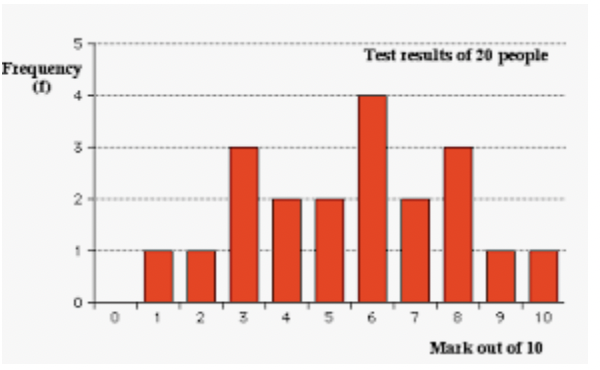
\includegraphics[width=0.7\textwidth]{Fig.4.1.jpg}
        \end{figure}
        \item Frequency diagram of continuous data - \textbf{\color{red}{Histogram}}
        \begin{figure}[H]
            \center
            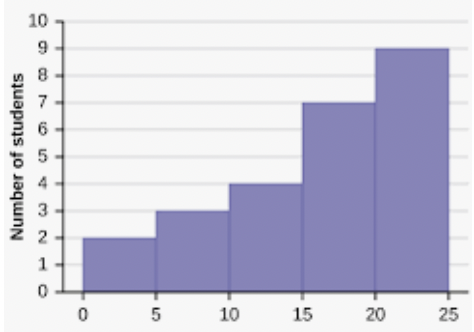
\includegraphics[width=0.7\textwidth]{Fig.4.2.jpg}
        \end{figure}
        \item Cumulative frequency table and cumulative frequency graph: 
        \begin{figure}[H]
            \center
            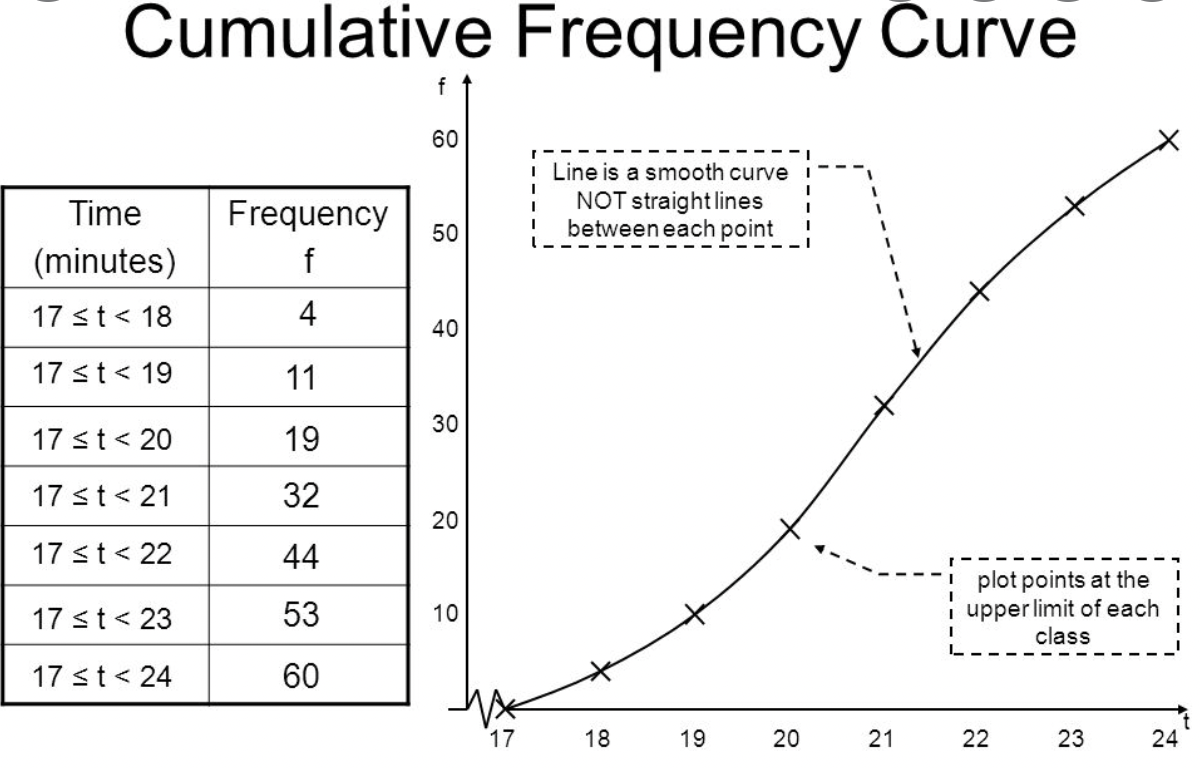
\includegraphics[width=0.7\textwidth]{Fig.4.3.jpg}
        \end{figure}
        \item For data grouped into intervals or classes, we can identify: 
        \begin{enumerate}
            \item Mid-interval values
            \item Interval width
            \item Lower interval boundaries
            \item Higher interval boundaries
            \item Modal class: the class with the highest frequency
        \end{enumerate}
    \end{itemize}
    \item Quartiles: 
    \begin{itemize}
        \item Minimum: the lowest value
        \item $Q_1$: the 25th percentile
        \item Median ($Q_2$): the 50th percentile
        \item $Q_3$: the 75th percentile
        \item Maximum: the highest value
        \item $${\color{red}{\text{Interquartile Range (IQR)}=Q_3-Q_1}}.$$ 
        \item Box-and-whisker plots: $\rightarrow$ spread of data: 
        \begin{figure}[H]
            \center
            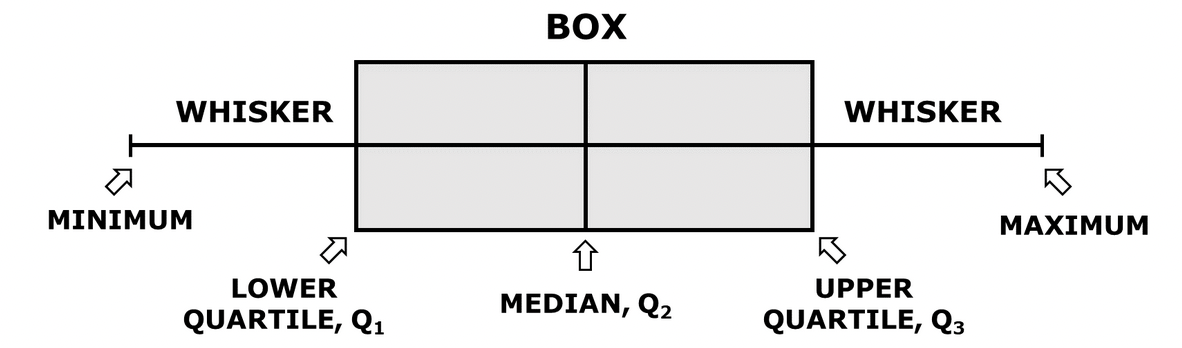
\includegraphics[width=0.7\textwidth]{Fig.4.4.jpg}
        \end{figure}
    \end{itemize}
    \item Normal distribution, negatively skewed, and positively skewed: 
    \item Normal distribution: $\text{mean}=\text{mode}=\text{median}$
    \item Positively skewed: $\text{median}<\text{mean}$
    \item Negatively skewed: $\text{median}>\text{mean}$
    \item Outliers: 
    $$\begin{aligned}
        &\color{red}\text{Ourlier}<Q_1-1.5\text{IQR}\\
    {\color{red}\text{OR}\quad}&{\color{red}\text{Outlier}>Q_3+1.5\text{IQR}}.
    \end{aligned}$$
    \item Measuring central tendency: 
    \begin{itemize}
        \item \begin{definition} \textbf{\color{red}{Mode}}: the value with the greatest frequency. \end{definition}
        \item \begin{definition}\textbf{\color{red}{Median}}({\color{red}{$m$}}): the middle value when the data is arranged in order.\end{definition}
        \item \begin{definition}\textbf{\color{red}{Mean}}({\color{red}{$\mu$}}): the arithmetic mean, the sum of the numerical data divided by the number of data points. 
        $${\color{red}{\mu=\frac{\sum^{n}_{i=1}x_i}{n}}}.$$\end{definition}
    \end{itemize}
    \item Measures of dispersion: 
    \begin{itemize}
        \item \begin{definition}Range: $${\color{red}{\text{Range}=x_\text{max}-x_\text{min}}}.$$\end{definition}
        \item \begin{definition}Interquartile Range (IQR): $${\color{red}{\text{IQR}=Q_3-Q_1}}.$$\end{definition}
        \item \begin{definition}Variance $\sigma^2$ and standard deviation $\sigma$: 
        $${\color{red}{\begin{aligned}
            \sigma^2&=\frac{\sum^k_{i=1}f_i\left(x_i-\mu\right)^2}{n}=\frac{\sum^k_{i=1}f_ix_i^2}{n}-\mu^2\\
            \sigma&=\sqrt{\sigma^2}
        \end{aligned}}}$$\end{definition}
    \end{itemize}
    \begin{proof}
        $$\begin{aligned}
            \sigma^2=\frac{\sum^k_{i=1}f_i\left(x_i-\mu\right)^2}{n}&=\frac{\sum^k_{i=1}f_ix_i^2}{n}-2\mu\frac{\sum^k_{i=1}f_ix_i}{n}+\mu^2\frac{\sum^k_{i=1}f_i}{n}\\
            &=\frac{\sum^k_{i=1}f_ix_i^2}{n}-2\mu^2+\mu^2\\
            &=\frac{\sum^k_{i=1}f_ix_i^2}{n}-\mu^2
        \end{aligned}$$
    \end{proof}
\end{enumerate}

\subsection{Linear Correlation of Bivariate Data}
\begin{enumerate}
    \item Scatter Plot
    \item Linear correlation: 
    \begin{itemize}
        \item \textbf{\color{red}{Positive linear correlation}}: the line as a general upward trend. 
        \item Negative correlation.
        \item Quadratic trend
        \item Exponential trend
    \end{itemize}
    \item Estimate a line of best fit: 
    \begin{theorem}
        The line must pass through the mean point of the data set $(\overline{x},\overline{y})$, where $\overline{x}$ is the mean of $x$ and $\overline{y}$ is the mean of $y$.
    \end{theorem}
    \item Pearson's correlation coefficient ($r$): 
    \begin{itemize}
        \item Range: $-1\leq r\leq 1$
        \begin{enumerate}
            \item $r=-1$: perfect negative linear correlation
            \item $r=1$: perfect positive linear correlation
            \item $r=0$: no linear correlation
            \item $0.7<\left|r\right|\leq 1$: strong linear correlation
            \item $0.3<\left|r\right|\leq 0.7$: weak to moderate linear correlation
        \end{enumerate}
        \item Formula: 
        $${\color{red}{\begin{aligned}
            r&=\frac{\sum\left(x-\overline{x}\right)\left(y-\overline{y}\right)}{\sqrt{\sum\left(x-\overline{x}\right)^2\sum\left(y-\overline{y}\right)^2}}\\
            r&=\frac{\sum xy-n\overline{x}\ \overline{y}}{\sqrt{\sum x^2-n\overline{x}^2}\sqrt{\sum y^2-b\overline{y}^2}}
        \end{aligned}}}$$
    \end{itemize}
    \item Prediction using the least square linear regression: 
    \begin{itemize}
        \item The dangers of extrapolation.
        \item We cannot always reliably make a prediction of $x$ from a value of $y$, using a $y$ on $x$ line. 
    \end{itemize}
\end{enumerate}

\subsection{Probability and Expected Outcomes}
\begin{enumerate}
    \item \begin{definition}\textbf{\color{red}{Random Events}}: although we don't know the exact result in advance, we do know the set of all possible results. \end{definition}
    \begin{itemize}
        \item The set of all possible results is called the \textbf{\color{red}{sample space}} ($U$). 
        \item The number of all possible outcomes that make up the sample space is denoted as ${\color{red}{n(U)}}$.
        \item Any subset of a sample space is called an \textbf{\color{red}{event}}. The event consists of one or more outcomes. 
        \item Each time an experiment is repeated, it is considered a \textbf{\color{red}{trial}} of the experiment. 
    \end{itemize}
    \item \textbf{\color{red}{Experimental probability}} (relative frequency) is found by repeating an experiment a number of times and counting the number of times that particular outcome occurs. 
    \item \begin{definition}\textbf{\color{red}{Mutually exclusive}}: two events that do not share any outcomes {\color{green}{$\rightarrow$ They cannot occur together.}}\end{definition}
    \item \begin{definition}\textbf{\color{red}{Theoretical probability}}: When running an experiment for $N$ trials that results in an event A occurring $n(A)$ times, the probability of $A$ happening, $\P(A)$ is $$\P(A)=\lim_{N\to\infty}\frac{n(A)}{N}.$$
    If an experiment has equally likely outcomes, the probability of event $A$ occurring is defined as $${\color{red}{\P(A)=\frac{n(A)}{n(U)}=\frac{\text{Number of outcomes in which A occurs}}{\text{Total number of outcomes in the sample space}}}}.$$\end{definition}
    \item Axioms:
    \begin{axiom}
        For any event $A$, $${\color{red}{0\leq \P(A)\leq 1}}.$$
    \end{axiom}
    \begin{axiom}
        The probability of nothing ($o$) occurring is zero: $${\color{red}{\P(o)=0}}.$$
        The probability of one of all the outcomes in the sample space occurring is one: $${\color{red}{\P(U)=1}}.$$
    \end{axiom}
    \begin{axiom}
        If $A$ and $B$ are $\in U$ and are mutually exclusive, then the probability of either $A$ or $B$ happening is $${\color{red}{\P(A\cup B)=\P(A)+\P(B)}}.$$
    \end{axiom}
    \begin{axiom}
        If $\P(A')$ is the probability of event $A$ not happening, $${\color{red}{\P(A')=1-\P(A)}},$$ where $\P(A)$ is the probability of event $A$ occurring. 
    \end{axiom}
    \item \begin{definition}Expectation: The formula for expected number of members of group $A$ in a sample of size $n$ is $${\color{red}{n\P(A)}}.$$\end{definition}
    {\color{green}{If choosing $n$ from the population, $n\P(A)$ gives an approximation of how many of them would be members of group $A$.}}
\end{enumerate}

\subsection{Probability Calculations}
\begin{enumerate}
    \item 
    \begin{definition} A \textbf{\color{red}{Venn diagram}} is a model illustrating two or more sets of data using overlapping circles to show elements of each set. 
        \begin{figure}[H]
            \center
            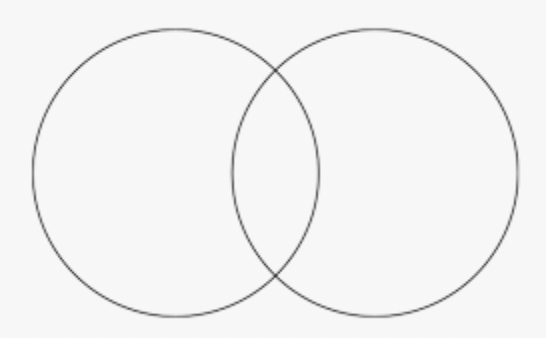
\includegraphics[width=0.7\textwidth]{Fig.4.5.jpg}
        \end{figure}
    \end{definition}
    \begin{itemize}
        \item \begin{definition}The probability of event $A$ and $B$ occurring at the same time: $$\P(A\cap B)$$\end{definition}
        \item \begin{definition}The probability of event $A$ or $B$ occurring ($A$ union $B$): $$\P(A\cup B)$$\end{definition}
        \item \begin{theorem}If $\P(A\cup B)=\varnothing$, then $A$ and $B$ are \textbf{mutually exclusive}.\end{theorem}
    \end{itemize}
    \item The tree diagram
    \item \begin{theorem}The probability of a union: $${\color{red}{\P(A\cup B)=\P(A)+\P(B)-\P(A\cap B)}}.$$\end{theorem}
    \begin{proof}
        $$n(A\cup B)=n(A)+n(B)-n(A\cap B),$$
        $$\begin{aligned}
            \P(A\cup B)=\frac{n(A\cup B)}{n(U)}&=\frac{n(A)+n(B)-n(A\cap B)}{n(U)}\\
            &=\P(A)+\P(B)-\P(A\cap B).
        \end{aligned}$$
    \end{proof}
    \item Conditional probability: 
    \begin{itemize}
        \item Conditional probability shrinks the sample space and, therefore, increases the probability of an event occurring, unless the given information renders the event impossible. 
        \item \begin{theorem} 
            $${\color{red}{\P(A|B)=\frac{\P(A\cap B)}{\P(B)}}},$$
            where $\P(A|B)$ is read as probability of event $A$ occurring, given event $B$ occurring. 
        \end{theorem}
        \begin{proof}
            If we know that $B$ has occurred, the sample space now contains all the elements of $B$ but no more. Now, we select events from the sample space that falls in $A$: 
            $$\begin{aligned}
                \P(A|B)&=\frac{n(A\cap B)}{n(B)}\\
                &=\frac{\frac{n(A\cap B)}{n(U)}}{\frac{n(B)}{n(U)}}=\frac{\P(A\cap B)}{\P(B)}.
            \end{aligned}$$
        \end{proof}
    \end{itemize}
    \item The probability of independent events: 
    \begin{itemize}
        \item \begin{definition}$A$ and $B$ are \textbf{\color{red}{independent events}} if the occurrence of $A$ has no effect on the probability of $B$ occurring. \end{definition}
        $${\color{red}{\P(B|A)=\P(B)}}\text{\quad OR\quad}{\color{red}{\P(A|B)=\P(A)}}.$$
        \item \begin{theorem} $A$ and $B$ are independent if and only if $${\color{red}{\P(A\cap B)=\P(A)\times \P(B)}}.$$\end{theorem}
    \end{itemize}
    \item \begin{theorem}Probability of union when $A$ and $B$are mutually exclusive: $${\color{red}{\P(A\cup B)=\P(A)+\P(B)}}.$$\end{theorem}
\end{enumerate}

\subsection{Discrete Random Variables}
\begin{enumerate}
    \item \begin{definition}If a random variable can take exactly $N$ values, each of which corresponds to a unique outcome in the sample space of an experiment, then this variable is a \textbf{\color{red}{discrete random variable}}.\end{definition}
    \begin{itemize}
        \item The probability that $x$ takes on any of the $N$ values is written as ${\color{red}{\P(X=x)}}$
        \item A \textbf{\color{red}{probability distribution}} is a combination of the sample space of a random experiment with the probabilities of each of the events in the sample space. 
        \item PDF: probability distribution function
        \item \begin{axiom}For each value $\{x_i\}$ of the random variable $X$, we have that $$0\leq \P(X=x_i)\leq 1.$$\end{axiom}
        \item \begin{axiom} As $X$ may take on any of the $N$ values of the sample space, the sum of the probabilities of each of them as an outcome of the experiment must equal one: $${\color{red}{\sum^N_{i=1}\P(X=x_i)=\P(X=x_1)+\P(X=x_2)+\P(X=x_3)+\cdots+\P(X=x_N)=1}}.$$\end{axiom}
        \item \begin{definition} \textbf{\color{red}{Well-defined probability distribution}}: a probability distribution that satisfies both $$\begin{cases}0\leq \P(X=x_i)\leq 1\\\sum^N_{i=1}\P(X=x_i)=1\end{cases}$$\end{definition}
    \end{itemize}
    \item Calculating expected value: 
    \begin{itemize}
        \item \begin{definition}The \textbf{\color{red}{expected value}} (expected mean) is the value you would expect to obtain on average if you performed an experiment many times. \end{definition}
        \item The expected value of a random variable $X$ with a probability distribution function $\P(X=x)$ is written as ${\color{red}{\E(X)}}$ or ${\color{red}{\mu}}$. 
        \item Formula: 
        $${\color{red}{\begin{aligned}
            \E(X)=\mu&=\sum^N_{i=1}x_i\P(X=x_i)\\
            &=x_1\P(X=x_1)+x_2\P(X=x_2)+x_3\P(X=x_3)+\cdots+x_N\P(X=x_N)
        \end{aligned}}}$$
        \item Application: fairness of a game\\
        A fair game is perfectly balanced so that the expected mean pay-out is $0$ for both players. 
    \end{itemize}
\end{enumerate}

\subsection{The Binomial Distribution}
\begin{enumerate}
    \item The binomial distribution discrete the probability distribution of different outcomes of repeated binary events. 
    \begin{itemize}
        \item Since there are only two outcomes, we use ${\color{red}{p}}$ to represent the probability of success, meaning the probability that the event we are looking for occurs. 
        \item We use ${\color{red}{X\sim}}$ to denote a random variable $X$ that is distributed in a certain way. 
        \item ${\color{red}{X\sim \mathrm{B}(n,p)}}$ represents the binomial distribution, \\
        where $mathrm{B}$ stands for binomial, $n$ represents the number of trials in the binomial experiment, and $p$ is the probability of success. 
        \item The probability of failure is $q$: $${\color{red}{q=1-p}}.$$
        \item \begin{theorem}Expected value of a binomial distribution: $${\color{red}{\E(X)=np}}.$$\end{theorem}
        \item \begin{theorem}Variance of a binomial distribution: $${\color{red}{\Var(X)=np(1-p)=npq}}.$$\end{theorem}
    \end{itemize}
    \item Probabilities within the binomial distribution: 
    \begin{theorem} A random variable that is binomially distributed and takes on the value of the number of success in $n$ trials is written as $X\sim\mathrm{B}(n,p)$, where $p$ is the probability of success in one trial. Then, the probability that $X$ takes on an actual value of $x$ successes is given by: 
    $${\color{red}{X\sim\mathrm{B}(n,p)\Rightarrow\P(X=x)=\binom{n}{x}p^x\left(1-p\right)^{n-x},\ x=0,1,2,3,\cdots,n}}.$$
    \end{theorem}
    \item Finding binomial probabilities using GDC: 
    \begin{itemize}
        \item \textbf{Binomial PDF} returns a specific value of $\P(X=x)$
        \item \textbf{Binomial CDP} (cumulative distribution function) gives the value of $$\P(0\leq X\leq \text{upper bound}).$$
        \item \begin{theorem}$${\color{red}{\P(a\leq X\leq b)=\P(0\leq X\leq b)-\P(0\leq X\leq a-1)}}.$$\end{theorem}
    \end{itemize}
\end{enumerate}

\subsection{The Normal Distribution and Curve}
\begin{enumerate}
    \item The normal (bell) curve: 
    \begin{itemize}
        \item The normal distribution is modeled graphically with a \textbf{\color{red}{normal curve}}: 
        \begin{figure}[H]
            \center
            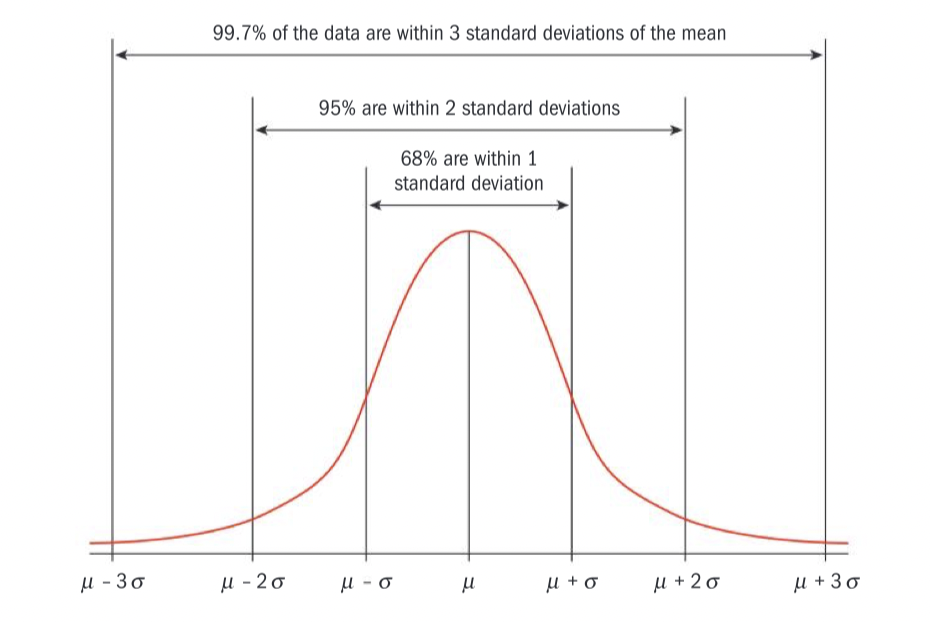
\includegraphics[width=0.8\textwidth]{Fig.4.6.jpg}
        \end{figure}
        \item The normal curve always has its highest point in the center, and that point is the mean ($\mu$), median, and mode. 
        \item The axis is often labeled using the standard deviation $\sigma$.
        \item The normal distribution deals with continuous random variables. 
    \end{itemize}
    \item Expressing the normal distribution algebraically: 
    \begin{itemize}
        \item Normal distribution is denoted as $${\color{red}{X\sim\mathrm{N}(\mu,\sigma^2)}},$$ where $\mathrm{N}$ means normal distribution, $\mu$ is the mean, and $\sigma$ is the standard deviation. 
        \item Normal probability density function: 
        \begin{enumerate}
            \item A probability density function is the equation of a curve that has the probabilities as the area underneath. 
            \item \begin{definition} For $X\sim\mathrm{N}(\mu,\sigma^2)$, 
            $${\color{red}{f(x)=\frac{1}{\sigma\sqrt{2\pi}}e^{-\frac{1}{2}\left(\frac{x-\mu}{\sigma}\right)^2},\text{ where }-\infty<x<\infty}}.$$
            $$\int_{-\infty}^\infty f(x) \d x=\int_{-\infty}^\infty \frac{1}{\sigma\sqrt{2\pi}}e^{-\frac{1}{2}\left(\frac{x-\mu}{\sigma}\right)^2}\d x=1.$$
            \end{definition}
        \end{enumerate}
    \end{itemize}
    \item Calculating normal distributed probabilities with GDC: 
    \begin{itemize}
        \item Normal PDF and Normal CDF.
        \item Inverse Normal Function.
    \end{itemize}
    \item Standard Normal Distribution: 
    \begin{itemize}
        \item Transform $X\sim\mathrm{N}(\mu,\sigma^2)$ into $Z\sim\mathrm{N}(0,1)$: 
        \begin{figure}[H]
            \center
            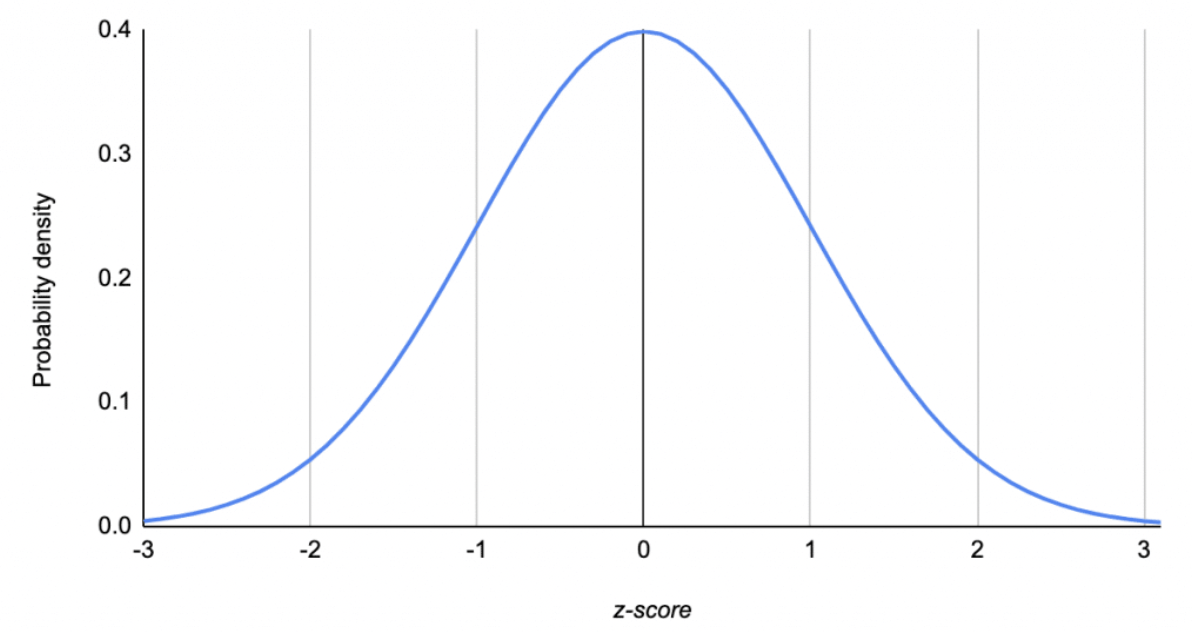
\includegraphics[width=0.8\textwidth]{Fig.4.7.jpg}
        \end{figure}
        \item Z-score: $${\color{red}{z=\frac{x-\mu}{\sigma}}}.$$
        \item Finding probabilities with z-scores: 
        \begin{enumerate}
            \item $$\P(-1<z<1)\approx 0.68$$
            $$\P(-2<z<2)\approx 0.95$$
            $$\P(-3<z<3)\approx 0.997$$
            \item Normal CDP on GDC
        \end{enumerate}
        \item Using z-score to find $\mu$ and $\sigma$.
    \end{itemize}
\end{enumerate}

\subsection{Probability Density Function (PDF)}
\begin{enumerate}
    \item For a \textbf{\color{red}{continuous random variable}} $X$ with \textbf{\color{red}{probability density function}} $f(x)$, it holds $$\begin{cases}f(x)\geq 0{\color{green}{\text{ \quad i.e., the function is non-negative}}}\\ \int_{-\infty}^{\infty}f(x)\d x=1{\color{green}{\text{ \quad i.e., the total area under the curve is 1}}}\end{cases}.$$
    \item The probability that $X$ takes values between $a$ and $b$ is $${\color{red}{\P(a\leq X\leq b)=\int_a^b f(x)\d x}}$$ {\color{green}{N.B.: $\P(a\leq X\leq b)=\P(a<X<b)$ because $\P(X=a)=0$.}}
    \item The \textbf{\color{red}{mean $\mu$}}, or the \textbf{\color{red}{expected value $\E(X)$}}, is defined by $${\color{red}{\mu=\E(x)=\int_{-\infty}^\infty xf(x)\d x}}.$$
    \item The \textbf{\color{red}{Variance $\Var(X)$}} is defined by $${\color{red}{\Var(X)=\E(X-\mu)^2=\int_{-\infty}^\infty(x-\mu)^2f(x)\d x}}.$$ An equivalent and more practical definition is $${\color{red}{\Var(X)=E(X^2)-\mu^2}}, \text{ where }\E(X^2)=\int_{-\infty}^\infty x^2f(x)\d x.$$
    \item Mode: the value of $x$ where $f(x)$ has its maximum. 
    \item Median: The value of $m$ where $\P(X\leq m)=0.5$
    \begin{example}
        $$\text{Let }f(x)=\begin{cases}f_1(x), a\leq x\leq b\\f_2(x), b<x\leq c\end{cases}, \text{ we check }\int_a^b f_1(x)\d x=A: $$
        \begin{enumerate}
            \item If $A>0.5$, the median $m\in\left[a,b\right]$, solve $$\int_a^mf_1(x)\d x=0.5.$$
            \item If $A<0.5$, the median $m\in\left[b,c\right]$, solve $$\int_m^cf_2(x)\d x=0.5.$$
        \end{enumerate}
    \end{example}
    \item Quartiles: 
    \begin{itemize}
        \item The \textbf{\color{red}{lower quartile $Q_1$}} is defined by $\P(X\leq Q_1)=0.25$, i.e., solve $$\int_{-\infty}^{Q_1}f(x)\d x=0.25.$$
        \item The \textbf{\color{red}{upper quartile $Q_3$}} is defined by $\P(X\leq Q_3)=0.75$, i.e., solve $$\int_{-\infty}^{Q_3}f(x)\d x=0.75.$$
    \end{itemize}
    \item The effects of linear transformations on the random variable $X$: 
    \begin{itemize}
        \item $${\color{red}{\E(aX+b)=a\E(X)+b}}.$$
        \item $${\color{red}{\Var(aX+b)=a^2\Var(X)}}.$$
    \end{itemize}
\end{enumerate}

\subsection{The Bayes' Theorem}
\begin{enumerate}
    \item Bayes' Theorem: 
    \begin{theorem}{Bayes' Theorem}
        $${\color{red}{\P(A|B)=\frac{\P(A)\P(B|A)}{\P(B)}}}.$$
    \end{theorem}
    \begin{proof}
        $$\P(A|B)=\frac{\P(A\cap B)}{\P(B)}\ \Rightarrow\ \P(A\cap B)=\P(A|B)P(B)$$
        $$P(B|A)=\frac{\P(B\cap A)}{\P(A)}\ \Rightarrow\ \P(B\cap A)=\P(B|A)P(A)$$
        $$\begin{aligned}
            \because&\  \P(A\cap B)=\P(B\cap B),\\
            \therefore&\  \P(A|B)P(B)=\P(B|A)P(A).\\
            \therefore&\  \P(A|B)=\frac{\P(A)\P(B|A)}{\P(B)}.
        \end{aligned}$$
    \end{proof}
    \item Other versions of the Bayes' theorem: 
    \begin{itemize}
        \item $${\color{red}{\P(B)=\P(A\cap B)+\P(A'\cap B)=\P(A)\P(B|A)+\P(A')\P(B|A')}}.$$
        \item Substitute $\P(B)$: 
        $$\begin{aligned}
            {\color{red}{\P(A|B)}}&{\color{red}{=\frac{\P(B|A)\P(A)}{\P(A)\P(B|A)+\P(A')\P(B|A')}}};\\
            \P(B|A)&=\frac{\P(A|B)\P(B)}{\P(B)\P(A|B)+\P(B')\P(A|B')}.
        \end{aligned}$$
    \end{itemize}
    \item Bayes' theorem for three events: 
    $$\begin{aligned}
        \P(B)&=\P(A_1\cap B)+\P(A_2\cap B)+\P(A_3\cap B)\\
        &=\P(A_1)\P(B|A_1)+\P(A_2)\P(B|A_2)+\P(A_3)\P(B|A_3).
    \end{aligned}$$
    $${\color{red}{\begin{aligned}
        {\color{black}{\therefore}}\ \P(A_i|B)&=\frac{\P(A_i)\P(B|A_i)}{\P(B)}\\
        &=\frac{\P(A_i)\P(B|A_i)}{\P(A_i)\P(B|A_i)+\P(A_2)\P(B|A_2)+\P(A_3)\P(B|A_3)}.
    \end{aligned}}}$$
\end{enumerate}

\end{document}